%!TEX program = lualatex
%!TEX encoding = UTF-8 Unicode  
%!TEX root = chapter16.tex  
\documentclass[main.tex]{subfiles}
\begin{document} 
%----------------------------------------------------------------------------------------
%	CHAPTER  16
%----------------------------------------------------------------------------------------
\cleardoublepage
\loadgeometry{marginlayout}  
\pagestyle{scrheadings} % Print headers again  
\KOMAoptions{
	headwidth=textwithmarginpar,
	headsepline=true,
	headsepline= 0.5pt,
	footwidth=textwithmarginpar,
}   
\onehalfspacing 
\setcounter{chapter}{15}
\chapter{Inéquations produit et quotient}
	 
Lors de l'étude de la fonction carré, nous avons appris à résoudre des équations se ramenant à $x^2\geqslant k$ ou similaire. Ce chapitre aborde une approche plus systématique qui s'adapte à des situations plus complexes.

 
%----------------------------------------------------------------------------------------
%	   
%----------------------------------------------------------------------------------------
					
										
														
\newpage 
\loadgeometry{marginlayout}  
\pagestyle{scrheadings} % Print headers again  
\KOMAoptions{
	headwidth=textwithmarginpar,
	headsepline=true,
	headsepline= 0.5pt,
	footwidth=textwithmarginpar,
} 
\onehalfspacing
\section{Signe d'expressions}
\begin{example}[Signe évident] \hfill 
	
\begin{enumerate}[label=\arabic*),leftmargin=*]
	\item Pour tout $x\in\mathbb{R}$ : $f(x)=9(8x-4)^2+7$ est strictement positive
	\item Pour tout $x\in\mathbb{R}$ : $g(x)=-7(9x+3)^2-3$ est strictement négative
	\item Pour tout $x\in\mathbb{R}$ : $h(x)=-8(3x-1)^2$ est négative. S'annulle pour $x=\frac{1}{3}$.
\end{enumerate} 
\end{example}
\begin{example}[Signe d'un produit] Étudier le signe de $f(x)=(9x+10)(3x+1)$ selon les valeurs de $x$.\medskip
	 
	\noindent	On dresse le tableau de signe du produit après avoir cherché ses zéros de chaque facteur :
	
	\noindent\hfill  	\begin{tikzpicture}
		\tikzset{  double style/.style = {double,thick,double distance=2pt}}
		\tkzTabInit[lgt = 4.0, espcl = 2.5, color, colorC = blue!15, colorL = green!15]{$x$ / 1 , $9x+10$ / 1 , $3x+1$/ 1, $(9x+10)(3x+1)$ / 1.5 }{$-\infty$,  ,   ,   $+\infty$}
		\tkzTabLine{t, ,t, ,t, ,t}
		\tkzTabLine{t, ,t, ,t, ,t}
		\tkzTabLine{t, ,t, ,t, ,t} 
	\end{tikzpicture} 
	
	On peut dire que $(9x+10)(3x+1)<0$ lorsque \dotfill 
\end{example}
\begin{example}[Signe d'un quotient] Étudier le signe de $f(x)=\frac{-3x+6}{9x+4}$ selon les valeurs de $x$.\medskip
	
	\noindent	Valeurs interdites : $9x+4\neq 0 \iff x\neq \qquad$. \\
	
	\noindent Le domaine de l'expression est\dotfill
	  
	\noindent	On dresse le tableau de signe du quotient après avoir cherché les zéros de chaque facteur :
	
	\noindent\hfill  	\begin{tikzpicture}
		\tikzset{  double style/.style = {double,thick,double distance=2pt}}
		\tkzTabInit[lgt = 3.0, espcl = 2.5, color, colorC = blue!15, colorL = green!15]{$x$ / 1 , $-3x+6$ / 1 , $9x+4$/ 1, $\frac{-3x+6}{9x+4}$ / 1.5 }{$-\infty$,  ,   ,   $+\infty$}
		\tkzTabLine{t, ,t, ,t, ,t}
		\tkzTabLine{t, ,t, ,t, ,t}
		\tkzTabLine{t, ,t, ,t, ,t} 
	\end{tikzpicture} 

On peut dire que $\frac{-3x+6}{9x+4}>0$ lorsque \dotfill 
\end{example}

%----------------------------------------------------------------------------------------
%	EXERCICES
%----------------------------------------------------------------------------------------

\newpage 
\loadgeometry{widelayout}  
\pagestyle{scrheadings} % Print headers again  
\KOMAoptions{
	headwidth=textwithmarginpar,
	headsepline=true,
	headsepline= 0.5pt,
	footwidth=textwithmarginpar,
} 
\onehalfspacing
\subsection{Exercices : tableaux de signes d'expressions}



\begin{exercise} Compléter les tableaux de signes suivants  \hfill 
	\vfill 
	\noindent
	\begin{tikzpicture}
		\tkzTabInit[lgt = 3.0, espcl = 2.5, color, colorC = blue!15, colorL = green!15]{$x$ / 1 , $2x-3$  / 1.0 ,     $(2x-3)^2$  / 1.5 }{$-\infty$,       ,  $+\infty$ }
		\tkzTabLine{ t,  ,t,   , t}      
		\tkzTabLine{ t,  ,t,   , t}  
	\end{tikzpicture}
	\hfill
	\begin{tikzpicture}
		\tkzTabInit[lgt = 3.0, espcl = 2.5, color, colorC = blue!15, colorL = green!15]{$x$ / 1 , $x-6$  / 1.0 ,     $\frac{1}{x-6}$  / 1.5 }{$-\infty$,       ,  $+\infty$ }
		\tkzTabLine{ t,  ,t,   , t}      
		\tkzTabLine{ t,  ,t,   , t}  
	\end{tikzpicture}
	
	
	\vfill 
	\noindent
	\begin{tikzpicture}
		\tkzTabInit[lgt = 3.0, espcl = 2.5, color, colorC = blue!15, colorL = green!15]{$x$ / 1 , $-3x-2$ / 1 , $-10$ / 1,  $-10(-3x-2) $ / 1.5 }{$-\infty$,       ,  $+\infty$ }
		\tkzTabLine{ t,  ,t,   , t}    
		\tkzTabLine{ t,  ,t,   , t}    
		\tkzTabLine{ t,  ,t,   , t}  
	\end{tikzpicture}
	\hfill
	\begin{tikzpicture}
		\tkzTabInit[lgt = 3.0, espcl = 2.5, color, colorC = blue!15, colorL = green!15]{$x$ / 1 ,$3x+2$ / 1 , $5$ / 1,  $\frac{5}{3x+2}$ / 1.5 }{$-\infty$,       ,  $+\infty$ }
		\tkzTabLine{ t,  ,t,   , t}    
		\tkzTabLine{ t,  ,t,   , t}    
		\tkzTabLine{ t,  ,t,   , t}  
	\end{tikzpicture}	
	
	\vfill 
	\noindent
	\begin{tikzpicture}
		\tkzTabInit[lgt = 3.0, espcl = 2.5, color, colorC = blue!15, colorL = green!15]{$x$ / 1 , $-3x-2$ / 1 ,  $-10(-3x-2)^2 $ / 1.5 }{$-\infty$,       ,  $+\infty$ }
		\tkzTabLine{ t,  ,t,   , t}     
		\tkzTabLine{ t,  ,t,   , t}  
	\end{tikzpicture}
	\hfill
	\begin{tikzpicture}
		\tkzTabInit[lgt = 3.0, espcl = 2.5, color, colorC = blue!15, colorL = green!15]{$x$ / 1 ,$3x+2$ / 1 ,   $\frac{5}{(3x+2)^2}$ / 1.5 }{$-\infty$,       ,  $+\infty$ }
		\tkzTabLine{ t,  ,t,   , t}    
		\tkzTabLine{ t,  ,t,   , t}  
	\end{tikzpicture}

\vfill 
	\noindent \begin{tikzpicture}			
	\tikzset{  double style/.style = {double,thick,double distance=2pt}}
	\tkzTabInit[lgt = 3, espcl = 2.5, color, colorC = blue!15, colorL = green!15]{$x$ / 1 ,  $5(-x+2)^2$  / 1.5 }{$-\infty$,     ,  $+\infty$ }     
	\tkzTabLine{ t,   ,t,    , t}  
\end{tikzpicture}
\hfill
\begin{tikzpicture}			
	\tikzset{  double style/.style = {double,thick,double distance=2pt}}
	\tkzTabInit[lgt = 3, espcl = 2.5, color, colorC = blue!15, colorL = green!15]{$x$ / 1 ,   $\frac{5}{-x+2}$ / 1.5 }{$-\infty$,      ,  $+\infty$ }     
	\tkzTabLine{ t,  ,t,    , t}  
\end{tikzpicture}	
\end{exercise}
 
 %----------------------------------------------------------------------------------------
 %	EXERCICES
 %----------------------------------------------------------------------------------------
 
 \newpage 
 
 \begin{exercise} Cochez les expressions dont le tableau de signe est donné. Plusieurs réponses sont possibles

\begin{multicols}{3}
\noindent	\begin{tikzpicture}			
	\tikzset{  double style/.style = {double,thick,double distance=2pt}}
	\tkzTabInit[lgt = 1.2, espcl = 2.0, color, colorC = blue!15, colorL = green!15]{$x$ / 1 ,  $A(x)$  / 1.5 }{$-\infty$,   $-2$   ,  $+\infty$ }     
	\tkzTabLine{ t, - ,z, +  , t}  
\end{tikzpicture}
\begin{enumerate}[label={\ding{111}\rule{0pt}{1.8em}},leftmargin=*]
	\item $-x-2$ 
	\item $-5(-x-2)$
	\item $(-x-2)^2$
	\item $-5(-x-2)^2$
	\item $\frac{1}{-x-2}$
	\item  $\frac{-5}{-x-2}$
	\item  $\frac{-5}{(-x-2)^2}$ 
\end{enumerate}

	\noindent 	 
	\begin{tikzpicture}			
		\tikzset{  double style/.style = {double,thick,double distance=2pt}}
		\tkzTabInit[lgt = 1.2, espcl = 2.0, color, colorC = blue!15, colorL = green!15]{$x$ / 1 ,  $B(x)$  / 1.5 }{$-\infty$,   $1$   ,  $+\infty$ }     
		\tkzTabLine{ t, - ,z, +  , t}  
	\end{tikzpicture}


\begin{enumerate}[label={\ding{111}\rule{0pt}{1.8em}},leftmargin=*]
	\item $-x+1$ 
	\item $9(-x+1)$
	\item $(-x+1)^2$
	\item $9(-x+1)^2$
	\item $\frac{1}{-x+1}$
	\item  $\frac{9}{-x+1}$
	\item  $\frac{9}{(-x+1)^2}$ 
\end{enumerate}

	\noindent 	 
	\begin{tikzpicture}			
	\tikzset{  double style/.style = {double,thick,double distance=2pt}}
	\tkzTabInit[lgt = 1.2, espcl = 2.0, color, colorC = blue!15, colorL = green!15]{$x$ / 1 ,  $C(x)$  / 1.5 }{$-\infty$,   $-\frac{10}{3} $   ,  $+\infty$ }     
	\tkzTabLine{ t, - ,z, -  , t}  
\end{tikzpicture}


	\begin{enumerate}[label={\ding{111}\rule{0pt}{1.8em}},leftmargin=*]
	\item $-3x-10$ 
	\item $-7(-3x-10)$
	\item $(-3x-10)^2$
	\item $-7(-3x-10)^2$
	\item $\frac{1}{-3x-10}$
	\item  $\frac{-7}{-3x-10}$
	\item  $\frac{-7}{(-3x-10)^2}$ 
\end{enumerate}
\end{multicols}
  
 	
 	\noindent 	\parbox{0.45\linewidth}{
 		\begin{tikzpicture}			
 			\tikzset{  double style/.style = {double,thick,double distance=2pt}}
 			\tkzTabInit[lgt = 2.5, espcl = 2.5, color, colorC = blue!15, colorL = green!15]{$x$ / 1 ,  $D(x)$  / 1.5 }{$-\infty$,   $-\frac{7}{2} $   ,  $+\infty$ }     
 			\tkzTabLine{ t, + ,d, +  , t}  
 		\end{tikzpicture}
 	}
 	\hfill \parbox{0.50\linewidth}{
 		\begin{multicols}{3}
 			\begin{enumerate}[label={\ding{111}\rule{0pt}{1.8em}},leftmargin=*]
 				\item $2x+7$ 
 				\item $3(2x+7)$
 				\item $(2x+7)^2$
 				\item $3(2x+7)^2$
 				\item $\frac{1}{2x+7}$
 				\item  $\frac{3}{2x+7}$
 				\item  $\frac{3}{(2x+7)^2}$ 
 			\end{enumerate}
 		\end{multicols} 	
 	}
 	
 \end{exercise}

% \newpage 
\begin{exercise} Pour chaque fonction, déterminer les zéros des facteurs et compléter son tableau de signe.
 	
% \begin{multicols}{3}
% 	\begin{enumerate}[label={\arabic*) },leftmargin=*]
% 		\item $f(x)= (-2x+3)(-3x-5) $ 
% 		\item $g(x)=(5x-65)(7-2x)$
% 		\item $h(x)=(2x+14)(6x+24)$
% 		\item $i(x)=(-3x-72)(-4x-96)$
% 		\item $j(x)=\frac{-x}{x+12}$
% 		\item $k(x)=\frac{2x-5}{7+21x}$
% 		\item $l(x)=\frac{x^2}{5x+3}$
% 		\item $u(x)=\frac{-14x+12}{x^2+3}$
% 		\item $v(x)=\frac{(x-1)(2x+1)}{1-9x}$ 
% 		\item $w(x)=\frac{5+x}{(x-6)(7x+8)}$ 
% 	\end{enumerate}
% \end{multicols} 
	
	\noindent\hfill  	\begin{tikzpicture}
	\tikzset{  double style/.style = {double,thick,double distance=2pt}}
	\tkzTabInit[lgt = 5.0, espcl = 2.5, color, colorC = blue!15, colorL = green!15]{$x$ / 1 ,   / 1 ,  / 1, $f(x)= (-2x+3)(-3x-5)$ / 1.5 }{$-\infty$,  ,   ,   $+\infty$}
	\tkzTabLine{t, ,t, ,t, ,t}
	\tkzTabLine{t, ,t, ,t, ,t}
	\tkzTabLine{t, ,t, ,t, ,t} 
\end{tikzpicture} 
\vfill

	\noindent\hfill  	\begin{tikzpicture}
	\tikzset{  double style/.style = {double,thick,double distance=2pt}}
	\tkzTabInit[lgt = 5.0, espcl = 2.5, color, colorC = blue!15, colorL = green!15]{$x$ / 1 ,   / 1 ,  / 1, $g(x)=(5x-65)(7-2x)$ / 1.5 }{$-\infty$,  ,   ,   $+\infty$}
	\tkzTabLine{t, ,t, ,t, ,t}
	\tkzTabLine{t, ,t, ,t, ,t}
	\tkzTabLine{t, ,t, ,t, ,t} 
\end{tikzpicture} 

	\noindent\hfill  	
\begin{tikzpicture}
	\tikzset{  double style/.style = {double,thick,double distance=2pt}}
	\tkzTabInit[lgt = 5.0, espcl = 2.5, color, colorC = blue!15, colorL = green!15]{$x$ / 1 ,   / 1 ,  / 1, $h(x)=(2x+14)(6x+24)$ / 1.5 }{$-\infty$,  ,   ,   $+\infty$}
	\tkzTabLine{t, ,t, ,t, ,t}
	\tkzTabLine{t, ,t, ,t, ,t}
	\tkzTabLine{t, ,t, ,t, ,t} 
\end{tikzpicture} 
\vfill

	\noindent\hfill  	\begin{tikzpicture}
	\tikzset{  double style/.style = {double,thick,double distance=2pt}}
	\tkzTabInit[lgt = 5.0, espcl = 2.5, color, colorC = blue!15, colorL = green!15]{$x$ / 1 ,   / 1 ,  / 1, $i(x)=(-3x-72)(-4x-96)$ / 1.5 }{$-\infty$,  ,   ,   $+\infty$}
	\tkzTabLine{t, ,t, ,t, ,t}
	\tkzTabLine{t, ,t, ,t, ,t}
	\tkzTabLine{t, ,t, ,t, ,t} 
\end{tikzpicture} 
\vfill

	\noindent\hfill  	\begin{tikzpicture}
	\tikzset{  double style/.style = {double,thick,double distance=2pt}}
	\tkzTabInit[lgt = 5.0, espcl = 2.5, color, colorC = blue!15, colorL = green!15]{$x$ / 1 ,   / 1 ,  / 1, $j(x)=\frac{-x}{x+12}$ / 1.5 }{$-\infty$,  ,   ,   $+\infty$}
	\tkzTabLine{t, ,t, ,t, ,t}
	\tkzTabLine{t, ,t, ,t, ,t}
	\tkzTabLine{t, ,t, ,t, ,t} 
\end{tikzpicture} 
\vfill

	\noindent\hfill  	\begin{tikzpicture}
	\tikzset{  double style/.style = {double,thick,double distance=2pt}}
	\tkzTabInit[lgt = 5.0, espcl = 2.5, color, colorC = blue!15, colorL = green!15]{$x$ / 1 ,   / 1 ,  / 1, $k(x)=\frac{2x-5}{7+21x}$ / 1.5 }{$-\infty$,  ,   ,   $+\infty$}
	\tkzTabLine{t, ,t, ,t, ,t}
	\tkzTabLine{t, ,t, ,t, ,t}
	\tkzTabLine{t, ,t, ,t, ,t} 
\end{tikzpicture} 
\vfill
\end{exercise}

\newpage 
  

	\noindent\hfill  	
\begin{tikzpicture}
	\tikzset{  double style/.style = {double,thick,double distance=2pt}}
	\tkzTabInit[lgt = 4.0, espcl = 2.5, color, colorC = blue!15, colorL = green!15]{$x$ / 1 ,   / 1 ,  / 1, $l(x)=\frac{x^2}{5x+3}$ / 1.5 }{$-\infty$,  ,   ,   $+\infty$}
	\tkzTabLine{t, ,t, ,t, ,t}
	\tkzTabLine{t, ,t, ,t, ,t}
	\tkzTabLine{t, ,t, ,t, ,t} 
\end{tikzpicture} 
\vfill 

	\noindent\hfill  	
\begin{tikzpicture}
	\tikzset{  double style/.style = {double,thick,double distance=2pt}}
	\tkzTabInit[lgt = 4.0, espcl = 2.5, color, colorC = blue!15, colorL = green!15]{$x$ / 1 ,   / 1 ,  / 1, $u(x)=\frac{-14x+12}{x^2+3}$ / 1.5 }{$-\infty$,  ,   ,   $+\infty$}
	\tkzTabLine{t, ,t, ,t, ,t}
	\tkzTabLine{t, ,t, ,t, ,t}
	\tkzTabLine{t, ,t, ,t, ,t} 
\end{tikzpicture} 

\vfill 

\noindent\hfill\begin{tikzpicture}
	\tkzTabInit[lgt = 5, espcl = 2.5, color, colorC = blue!15, colorL = green!15]{$x$ / 1 ,   \hfill  \null / 1 ,  \hfill   \null / 1,  \hfill   \null / 1, $v(x)=\frac{(x-1)(2x+1)}{1-9x}$  \hfill \null  / 1.2 }{$-\infty$,   ,  , ,  $+\infty$ }
	\tkzTabLine{ t,  ,t, ,t,  , t,  , t}  
	\tkzTabLine{ t,  ,t, ,t,  , t,  , t}   
	\tkzTabLine{ t,  ,t, ,t,  , t,  , t}   
	\tkzTabLine{ t,  ,t, ,t,  , t,  , t}  
\end{tikzpicture}

\vfill 

\noindent\hfill
\begin{tikzpicture}
	\tkzTabInit[lgt = 5, espcl = 2.5, color, colorC = blue!15, colorL = green!15]{$x$ / 1 ,   \hfill  \null / 1 ,  \hfill   \null / 1,  \hfill   \null / 1, $w(x)=\frac{5+x}{(x-6)(7x+8)}$  \hfill \null  / 1.2 }{$-\infty$,   ,  , ,  $+\infty$ }
	\tkzTabLine{ t,  ,t, ,t,  , t,  , t}  
	\tkzTabLine{ t,  ,t, ,t,  , t,  , t}   
	\tkzTabLine{ t,  ,t, ,t,  , t,  , t}   
	\tkzTabLine{ t,  ,t, ,t,  , t,  , t}  
\end{tikzpicture}
\vfill 
 


%----------------------------------------------------------------------------------------
%	 
%---------------------------------------------------------------------------------------- 
\newpage 
\loadgeometry{widelayout}  
\pagestyle{scrheadings} % Print headers again  
\KOMAoptions{
		headwidth=textwithmarginpar,
		headsepline=true,
		headsepline= 0.5pt,
		footwidth=textwithmarginpar,
	} 
\onehalfspacing
\section{Application à la résolution d'inéquations : exemples guidés} 

\begin{example} 
	Résoudre dans $\mathbb{R}$ l'inéquation $x^2\leqslant 4$ inconnue $x$.\footnote{Nous allons retrouver le résultat connu $\mathscr{S}=\interval{-2}{2}$} 
	
	%\noindent \parbox{0.45\linewidth}{
		$\begin{WithArrows}
			x^2&\leqslant 4 \Arrow{On transforme en une comparaison à zéro}\\
			\rule{0pt}{1.8em}	\iff\quad\qquad\qquad\qquad &\leqslant0\Arrow{On factorise le membre non nul}\\
			\rule{0pt}{1.8em}	\iff\qquad\qquad\qquad\qquad& \leqslant 0 
		\end{WithArrows}$ 
		
		On dresse le tableau de signe de la forme factorisée après avoir cherché ses zéros :
		
		\noindent\hfill  \begin{tikzpicture}
			\tikzset{  double style/.style = {double,thick,double distance=2pt}}
			\tkzTabInit[lgt = 3.5, espcl = 2.0, color, colorC = blue!15, colorL = green!15]{$x$ / 1 ,   / 1 ,  / 1,  / 1 }{$-\infty$,  ,   ,   $+\infty$}
			\tkzTabLine{t, ,t, ,t, ,t}
			\tkzTabLine{t, ,t, ,t, ,t}
			\tkzTabLine{t, ,t, ,t, ,t} 
		\end{tikzpicture}
		
		$\begin{WithArrows} 
			\iff\quad	\qquad\qquad&\leqslant 0 \Arrow{On utilise le tableau de signe de la forme factorisée}\\ 
			\mathscr{S}& = 
		\end{WithArrows}$ 
		%} 
\end{example}
\begin{example} 
	Résoudre dans $\mathbb{R}$ l'inéquation $x^2>5x$ inconnue $x$.
	
	%\noindent \parbox{0.45\linewidth}{
		$\begin{WithArrows}
			x^2&> 5x \Arrow{On transforme en une comparaison à zéro}\\
			\iff\quad	x^2-5x&>0\Arrow{On factorise le membre non nul}\\
			\iff\quad	x(x-5)& > 0 
		\end{WithArrows}$ 
		
		On dresse le tableau de signe de la forme factorisée après avoir cherché ses zéros :
		
		\noindent\hfill  \begin{tikzpicture}
			\tikzset{  double style/.style = {double,thick,double distance=2pt}}
			\tkzTabInit[lgt = 3.5, espcl = 2.0, color, colorC = blue!15, colorL = green!15]{$x$ / 1 , $x$ / 1 , $x-5$/ 1, $x(x-5)$ / 1 }{$-\infty$,  ,   ,   $+\infty$}
			\tkzTabLine{t, ,t, ,t, ,t}
			\tkzTabLine{t, ,t, ,t, ,t}
			\tkzTabLine{t, ,t, ,t, ,t} 
		\end{tikzpicture}
		
		$\begin{WithArrows} 
			\iff\quad	x(x-5)& > 0 \Arrow{On utilise le tableau de signe de la forme factorisée}\\
			\iff\quad x&\in \qquad \qquad \qquad \qquad\qquad\qquad \\
			\mathscr{S}& = 
		\end{WithArrows}$ 
		%} 
\end{example}
\begin{example} 
	Résoudre dans $\mathbb{R}$ l'inéquation $-5(x-2)^2\geqslant 7$ inconnue $x$.
	
	%\noindent \parbox{0.45\linewidth}{
		$\begin{WithArrows}
			-5(x-2)^2&\geqslant 7 \Arrow{On transforme en une comparaison à zéro}\\
			\iff\quad\qquad\qquad\qquad & \geqslant 0  \Arrow{Expression avec signe évident}\\
			\mathscr{S}& = \qquad\qquad
		\end{WithArrows}$ 
	\end{example}

\newpage
\begin{example} 
	Résoudre dans $\mathbb{R}$ l'inéquation $\frac{-3x+9}{-4x+7}<0$ inconnue $x$. \medskip
	
	
		\noindent	Valeurs interdites : $-4x+7= 0 \iff x\neq \qquad$. Le domaine de résolution est\dotfill\bigskip
	
		\noindent	\ding{52} comparaison à zéro \qquad \ding{52} même dénominateur \qquad \ding{52} facteurs affines  
		
	 \noindent On dresse le tableau de signe du quotient après avoir cherché les zéros des facteurs :
	 
		
		\noindent\hfill  \begin{tikzpicture}
			\tikzset{  double style/.style = {double,thick,double distance=2pt}}
			\tkzTabInit[lgt = 3.5, espcl = 2.0, color, colorC = blue!15, colorL = green!15]{$x$ / 1 , $-3x+9$  / 1 ,$-4x+7$  / 1,  $\frac{-3x+9}{-4x+7}$/ 1 }{$-\infty$,  ,   ,   $+\infty$}
			\tkzTabLine{t, ,t, ,t, ,t}
			\tkzTabLine{t, ,t, ,t, ,t}
			\tkzTabLine{t, ,t, ,t, ,t} 
		\end{tikzpicture}
		
		$\begin{WithArrows} 
%			 \frac{-3x+9}{-4x+7}&< 0 \qquad\qquad\qquad\qquad\Arrow{On utilise le tableau de signe}\\ 
			\mathscr{S}& = 
		\end{WithArrows}$ 
		%} 
\end{example}
\begin{example} Donner l'ensemble des solutions de  l'inéquation $\frac{-3x+9}{-4x+7}\geqslant0  $ inconnue $x$.
	\[
	\mathscr{S}= 	
	\]
\end{example}
\begin{example} 
	Résoudre dans $\mathbb{R}$ l'inéquation $\frac{x^2+4x}{2x^2+3}>0$ inconnue $x$.\medskip
	
	\noindent	Valeurs interdites : \dotfill \bigskip
	
		\noindent	\ding{52} comparaison à zéro \qquad \ding{52} même dénominateur \qquad \ding{53} facteurs affines  
		
		
	\noindent	$\begin{WithArrows}
		\frac{x^2+4x}{2x^2+3}&>0\Arrow{On factorise au maximum}\\ 
		\rule{0pt}{1.8em}	\iff\quad\qquad\qquad\qquad & >0  \quad \text{\ding{52} facteurs affines ou signe évident} 
	\end{WithArrows}$ \bigskip
	
	 \noindent On dresse le tableau de signe du quotient après avoir cherché les zéros des facteurs :
	
	\noindent\hfill  	\begin{tikzpicture}
		\tikzset{  double style/.style = {double,thick,double distance=2pt}}
		\tkzTabInit[lgt = 3.5, espcl = 2.5, color, colorC = blue!15, colorL = green!15]{$x$ / 1 ,   / 1 ,  / 1 ,  / 1,   / 1.5 }{$-\infty$,  ,   ,   $+\infty$}
		\tkzTabLine{t, ,t, ,t, ,t}
		\tkzTabLine{t, ,t, ,t, ,t}
		\tkzTabLine{t, ,t, ,t, ,t}
		\tkzTabLine{t, ,t, ,t, ,t} 
	\end{tikzpicture}
	
	$\mathscr{S}=$ 
\end{example}
\vfill
\begin{eBox}
\textbf{à retenir : } On résout des inéquations sous la forme de comparaison à zéro en dressant le tableau de signe de la forme factorisée au maximum !
\end{eBox}
\newpage
\begin{example} 
	Résoudre dans $\mathbb{R}$ l'inéquation $\frac{1}{4x-3}\geqslant2$ inconnue $x$.\medskip
	
	\noindent	Valeurs interdites : \dotfill \bigskip
	
	\noindent	$\begin{WithArrows}
		\frac{1}{4x-3}&\geqslant2\Arrow{On transforme en une comparaison à zéro}\\
		\rule{0pt}{1.8em}	\iff\quad\qquad\qquad\qquad & \geqslant 0\Arrow{On ramène au même dénominateur le membre non nul}[jump=2]\\
		\rule{0pt}{1.8em}	\iff\quad\qquad\qquad\qquad &  \geqslant 0 \\
		\rule{0pt}{1.8em}	\iff\quad\qquad\qquad\qquad &  \geqslant 0  \quad \text{\ding{52} facteurs affines} 
	\end{WithArrows}$ \bigskip
	
	% \noindent On dresse le tableau de signe du quotient après avoir cherché ses racines :
	
	\noindent\hfill  	\begin{tikzpicture}
		\tikzset{  double style/.style = {double,thick,double distance=2pt}}
		\tkzTabInit[lgt = 3.5, espcl = 2.5, color, colorC = blue!15, colorL = green!15]{$x$ / 1 ,   / 1 ,  / 1,   / 1.5 }{$-\infty$,  ,   ,   $+\infty$}
		\tkzTabLine{t, ,t, ,t, ,t}
		\tkzTabLine{t, ,t, ,t, ,t}
		\tkzTabLine{t, ,t, ,t, ,t} 
	\end{tikzpicture}
	
	$\mathscr{S}=$ 
\end{example}

\begin{example} 
	Résoudre dans $\mathbb{R}$ l'inéquation $\frac{1}{4x+3}\geqslant \frac{2}{x}$ inconnue $x$.\medskip
	
	\noindent	Valeurs interdites : \dotfill \bigskip
	
	\noindent	$\begin{WithArrows}
		\frac{1}{4x+3}&\geqslant\frac{2}{x}\Arrow{On transforme en une comparaison à zéro}\\
		\rule{0pt}{1.7em}	\iff\quad\quad\quad\quad\qquad\qquad\qquad & \geqslant 0\Arrow{On ramène au même dénominateur}[jump=3]\\
		\rule{0pt}{1.8em}	\iff\quad\quad\quad\quad\quad\qquad\qquad\qquad &  \geqslant 0 \\
		\rule{0pt}{1.8em}	\iff\quad\quad\quad\quad\quad\qquad\qquad\qquad &  \geqslant 0 \\
		\rule{0pt}{1.8em}	\iff\quad\quad\quad\quad\quad\qquad\qquad\qquad &  \geqslant 0  \quad \text{\ding{52} facteurs affines}.
	\end{WithArrows}$  \bigskip
	%\noindent On dresse le tableau de signe du quotient après avoir cherché ses racines :
	
	\noindent\hfill  	\begin{tikzpicture}
		\tikzset{  double style/.style = {double,thick,double distance=2pt}}
		\tkzTabInit[lgt = 3.5, espcl = 2.0, color, colorC = blue!15, colorL = green!15]{$x$ / 1 ,   / 1 ,   / 1 , / 1,   / 1.5 }{$-\infty$,  , ,  ,   $+\infty$}
		\tkzTabLine{t, ,t, ,t, ,t, ,t}
		\tkzTabLine{t, ,t, ,t, ,t, ,t}
		\tkzTabLine{t, ,t, ,t, ,t, ,t}
		\tkzTabLine{t, ,t, ,t, ,t, ,t} 
	\end{tikzpicture}
	
	$\mathscr{S}=$ 
\end{example}
%----------------------------------------------------------------------------------------
%	EXERCICES
%----------------------------------------------------------------------------------------

\newpage 
\loadgeometry{widelayout}  
\pagestyle{scrheadings} % Print headers again  
\KOMAoptions{
	headwidth=textwithmarginpar,
	headsepline=true,
	headsepline= 0.5pt,
	footwidth=textwithmarginpar,
} 
\onehalfspacing
\subsection{Exercices : résolution d'inéquations à l'aide de tableaux de signes}
\begin{tBox}[frametitle={Point méthode}] 
 	\begin{enumerate} 
	\item Pour les inéquations rationnelles, préciser le domaine de résolution (valeurs interdites).
	\item  Vous ramènerez l'inéquation à une \textbf{comparaison à zéro} (i.e. une étude de signe)
	\item Déterminer la forme factorisée du membre non nul.
	\item Pour les inéquations rationnelles (avec des quotients) mettre au même dénominateur et factoriser numérateurs et dénominateurs si nécessaire.
	\item Vous chercherez les racines des termes affines de la forme \textbf{factorisée}. 
	\item Dresser le tableau de signe de la forme factorisée 
	\item  Conclure.
\end{enumerate}
\end{tBox}
\begin{exercise}\label{chapter15:exercice:inequation01}] Résoudre dans $\mathbb{R}$ les inéquations suivantes.\vspace{-1em} 
	\begin{multicols}{2}
		\begin{enumerate}[label={$(I_{\arabic*})$\rule{0pt}{1.6em} : },leftmargin=*]
			\item $(2x+5)(x-4)(-x-8)<0$
			\item $(x+1)^2(5x-3)\leqslant 0$
			\item $3x(x+3)-(x+3)^2 < 0$
			\item $ x^3+2x^2+x\geqslant 0$ 
			\item $(4x^ 2-9)(x+1)>0$
			\item $(2x-\sqrt{3})(x-\sqrt{2})>0$
		\end{enumerate}
	\end{multicols} 
\end{exercise}

\begin{exercise}\label{chapter15:exercice:inequation02}] Résoudre dans $\mathbb{R}$ les inéquations suivantes.\vspace{-1em} 
	\begin{multicols}{2}
		\begin{enumerate}[label={$(I_{\arabic*})$\rule{0pt}{1.6em} : },leftmargin=*]
			\item $x^2-4x\leqslant -2x-1$
			\item $(2x+3)^ 2>(2x+3)(x-3)$
			\item $(x+1)(x-3)\geqslant x^2-9$
			\item $ x^2-4+(x+2)(2x+5)<0$
		\end{enumerate}
	\end{multicols} 
\end{exercise}

\begin{exercise}\label{chapter15:exercice:inequation03}] Résoudre dans $\mathbb{R}$ les inéquations suivantes.\vspace{-1em} 
	\begin{multicols}{2}
		\begin{enumerate}[label={$(I_{\arabic*})$\rule{0pt}{1.6em} : },leftmargin=*]
			\item $\frac{2x-4}{x+2}>0$
			\item $\frac{-2x+8}{3x-2}<0$
			\item $\frac{2x^ 2}{-(x+1)(x+3)}\geqslant 0$
			\item $\frac{(x+1)(x-2)}{x^ 2+2}\leqslant 0$
			\item $\frac{-5x}{(2x-7)^2}\geqslant 0$
			\item $\frac{1+2x^2}{7-x}\geqslant 0$
		\end{enumerate}
	\end{multicols} 
\end{exercise}
\begin{exercise}\label{chapter15:exercice:inequation04}] Résoudre dans $\mathbb{R}$ les inéquations suivantes.\vspace{-1em} 
	\begin{multicols}{2}
		\begin{enumerate}[label={$(I_{\arabic*})$\rule{0pt}{1.6em} : },leftmargin=*] 
			\item $\frac{3x+1}{6-5x}\geqslant 2$
			\item $\frac{3x+1}{5-2x}\leqslant -3$
			\item $\frac{3}{x+1}>\frac{2}{x-1}$
			\item $\frac{x+5}{x-1}\leqslant \frac{x-3}{x+2}$
		\end{enumerate}
	\end{multicols} 
\end{exercise}
\begin{proof} [solution de l'exercice  \ref{chapter15:exercice:inequation01}]\scriptsize  
%\begin{multicols}{2} 
\begin{pycode}
from re import sub
import sympy as sp
from sympy.core.sympify import kernS
from sympy.solvers.inequalities import solve_univariate_inequality

x, y, z, t , a, b = sp.symbols('x y z t a b', real=True)
k, m, n = sp.symbols('k m n', integer=True)
f, g, h = sp.symbols('f g h', cls=sp.Function)

# Create a list of functions to include in the table
funcs = [  
(2*x+5)*(x-4)*(-x-8)<0,
(x+1)**2*(5*x-3)<=0,
2*x*(x+3)-(x+3)**2<0,
x**3+2*x**2+x>=0,
(4*x**2-9)*(x+1)>0,
(2*x-sp.sqrt(3))*(x-sp.sqrt(2))>0,
]
n=1
#print(r'\begin{enumerate}[label={$(I_{\arabic*})$}] ')
for func in funcs:
	#print('\item ')
	print( '$\mathscr{S}_' + str(n)+ ' = ' + sp.latex(solve_univariate_inequality(func,   x,   domain=sp.S.Reals, relational=False)).replace("(", "]").replace(")", "[")   + '$'     )
	n = n + 1
#print(r'\end{enumerate}')
\end{pycode}
%\end{multicols}	
\end{proof}


\begin{proof}[solution de l'exercice  \ref{chapter15:exercice:inequation02}]\scriptsize   
%\begin{multicols}{2} 
\begin{pycode}
from re import sub
import sympy as sp
from sympy.core.sympify import kernS
from sympy.solvers.inequalities import solve_univariate_inequality

x, y, z, t , a, b = sp.symbols('x y z t a b', real=True)
k, m, n = sp.symbols('k m n', integer=True)
f, g, h = sp.symbols('f g h', cls=sp.Function)

# Create a list of functions to include in the table
funcs = [  
x**2-4*x<=-2*x-1,
(2*x+3)**2>(2*x+3)*(x-3),
(x+1)*(x-3)>=x**2-9,
x**2-4+(x+2)*(2*x+5)<0,
]
n=1 
for func in funcs: 
	print( '$\mathscr{S}_' + str(n)+ ' = ' + sp.latex(solve_univariate_inequality(func,   x, domain=sp.S.Reals, relational=False)).replace("(", "]").replace(")", "[")   + '$'     )
	n = n + 1
\end{pycode}
%\end{multicols}
\end{proof}


\begin{proof}[solution de l'exercice  \ref{chapter15:exercice:inequation03}]\scriptsize   
\begin{pycode}
from re import sub
import sympy as sp
from sympy.core.sympify import kernS
from sympy.solvers.inequalities import solve_univariate_inequality

x, y, z, t , a, b = sp.symbols('x y z t a b', real=True)
k, m, n = sp.symbols('k m n', integer=True)
f, g, h = sp.symbols('f g h', cls=sp.Function)

# Create a list of functions to include in the table
funcs = [  
(2*x-4)/(x+2)>0,
(-2*x+8)/(3*x-2)<0,
2*x**2/((-x-1)*(x+3))>-0,
(x+1)*(x-2)/(x**2+2)<=0,
-5*x/(2*x-7)**2>=0,
(1+2*x**2)/(7-x)>=0,
]
n=1 
for func in funcs: 
	print( '$\mathscr{S}_' + str(n)+ ' = ' + sp.latex(solve_univariate_inequality(func,   x,   domain=sp.S.Reals, relational=False)).replace("(", "]").replace(")", "[")   + '$'     )
	n = n + 1 
\end{pycode} 
% 
\end{proof}


\begin{proof}[solution de l'exercice  \ref{chapter15:exercice:inequation04}]\scriptsize   
\begin{pycode}
from re import sub
import sympy as sp
from sympy.core.sympify import kernS
from sympy.solvers.inequalities import solve_univariate_inequality

x, y, z, t , a, b = sp.symbols('x y z t a b', real=True)
k, m, n = sp.symbols('k m n', integer=True)
f, g, h = sp.symbols('f g h', cls=sp.Function)

# Create a list of functions to include in the table
funcs = [  
(3*x+1)/(6-5*x)>=2,
(3*x+1)/(5-2*x)<=-3,
3/(x+1)>2/(x-1),
(x+5)/(x-1)<=(x-3)/(x+2),
]
n=1 
for func in funcs: 
	print( '$\mathscr{S}_' + str(n)+ ' = ' + sp.latex(solve_univariate_inequality(func,   x,   domain=sp.S.Reals, relational=False)).replace("(", "]").replace(")", "[")   + '$'     )
	n = n + 1 
\end{pycode} 
% 	
\end{proof}


%----------------------------------------------------------------------------------------
%	 
%----------------------------------------------------------------------------------------
 
\newpage 
\loadgeometry{widelayout}  
\pagestyle{scrheadings} % Print headers again  
\KOMAoptions{
	headwidth=textwithmarginpar,
	headsepline=true,
	headsepline= 0.5pt,
	footwidth=textwithmarginpar,
} 
\onehalfspacing 
 
 
\section{Club de Maths : un carré est positif et applications}

\begin{eBox}
	Un grand nombre de résultats reposent sur le principe simple suivant : le carré d’un réel est un réel positif, et ce carré est nul si et seulement si le réel est nul. Dans cette feuille, nous explorons plusieurs 
	applications (simples et moins simples) de ce principe.
%	(\footnote{À partir d'un recueil du club de Maths de Nancy}).
	\end{eBox}

\begin{problem}[Petites astuces à connaître]\label{chapter08:problem:00} \hfill 
	
	 Montrer les inégalités suivantes sont vraies pour tout $a$ et $b\in\mathbb{R}$ :
	$$
	2ab\leqslant a^2+b^2
	\qquad\qquad 
	ab\leqslant \frac{(a+b)^2}{4}
	\qquad\qquad 
	(a+b)^2\leqslant 2(a^2+b^2)
	$$ 
\end{problem} 

\begin{problem}[Inégalité arithmético-géométrique]\label{chapter08:problem:03}\hfill

 \noindent\parbox{0.45\linewidth}{
	\begin{enumerate}[label=\alph*), leftmargin=*]
		\item Montrer que la figure ci-contre illustre l'inégalité pour $a, b\geqslant 0$, on a $$\sqrt{ab}\leqslant \frac{a+b}{2}$$
		\item Démontrer algébriquement l'inégalité précédente.
	\end{enumerate}
}\hfill
\parbox{0.5\linewidth}{
		\begin{tikzpicture}[scale=0.95]
			\def \b{2.3};
			\def \a{1.7}; 
			\def \c{5.0}; 
			\tkzDefPoint(0,0){A1}
			\tkzDefPoint(\a,0){A2}
			\tkzDefPoint(\a,\a){A3}
			\tkzDefPoint(\a+\b,0){A4}
			\tkzDefPoint(\a+\b,\a){A5}
			\tkzDefPoint(\a+\b,\a+\b){A6}
			\tkzDrawPolygon[ line width=1.2pt, fill=gray!10](A1,A2,A3)
			\tkzDrawPolygon[ line width=1.0pt](A2,A3,A5,A4)
			\tkzDrawPolygon[ line width=1.2pt, fill=gray!50](A3,A5,A6) 
			\tkzLabelSegment[below](A1,A2){\scriptsize $\sqrt{a}$} 
			\tkzLabelSegment[right](A4,A5){\scriptsize $\sqrt{a}$} 
			\tkzLabelSegment[right](A2,A3){\scriptsize $\sqrt{a}$} 
			\tkzLabelSegment[below](A3,A5){\scriptsize $\sqrt{b}$} 
			\tkzLabelSegment[right](A5,A6){\scriptsize $\sqrt{b}$} 
			\tkzLabelSegment[below](A2,A4){\scriptsize $\sqrt{b}$}
			
			\tkzDefPoint(\c+\a+\a,0){B1}
			\tkzDefPoint(\c+\a,0){B2}
			\tkzDefPoint(\c+\a,\a){B3}
			\tkzDefPoint(\c+\a+\b,0){B4}
			\tkzDefPoint(\c+\a+\b,\a){B5}
			\tkzDefPoint(\c+\a+\b,\a-\b){B6}
			\tkzDrawPolygon[ line width=1.2pt, fill=gray!10](B1,B2,B3)
			\tkzDrawPolygon[ line width=1.2pt, fill=gray!50](B3,B5,B6) 
			\tkzDrawPolygon[ line width=1.2pt, dashed](B2,B3,B5,B4) 
			\tkzDefPoint(\a*0.8,0){P}
			\tkzDefPoint(\a*1.2,0){Q}
			\tkzDefPoint(\a+\b,\a*1.2){R}
			\tkzDefPoint(\a+\b,\a*0.8){S}	
			\draw[line width=1.2pt,->,>=latex] (P) to[bend right=90] (Q);
			\draw[line width=1.2pt,->,>=latex] (R) to[bend left=90] (S);
			
			%			\tkzText[color = black, below, fill=white, text width=2.5cm](\c+1*\a+0.5*\b,\a+\b){\scriptsize de Y. Kobayashi  Soka University}	 
		\end{tikzpicture}
 }   
\end{problem}  
\begin{problem}[Inégalité de Cauchy-Schwarz et application]\label{chapter08:problem:04}\hfill

\begin{enumerate}[label=\alph*), leftmargin=*]
	\item Montrer que pour tout $x, y, u, v\in\mathbb{R}$ :
	$$(x^2+y^2)(a^2+b^2) \geqslant \big(xa +yb\big)^2$$
	\item En déduire pour $a>0$ et $b>0$ on a :
	$$(a+b)\left(\frac{1}{a}+\frac{1}{b}\right)\geqslant 4 $$
\end{enumerate}
\end{problem} 

 
\begin{problem}[Lemme du tourniquet]\label{chapter08:problem:05} 
Montrer que pour tout $a,b$ et $c\in\mathbb{R}$ on a :
	$$
	ab+bc+ca\leqslant a^2+b^2+c^2
	$$
et que s'il y a égalité alors les trois réels sont égaux. 
\end{problem}
  
\begin{proof}[solution du problème \ref{chapter08:problem:00}]
	Il s’agit de montrer que la différence est positive. Quelle est cette différence ? Peut-on
	l’écrire sous forme factorisée ?
\end{proof}
 

\begin{proof}[solution du problème \ref{chapter08:problem:04}]
	Il s’agit de montrer que la différence est positive. Quelle est cette différence ? Peut-on	l’écrire sous forme factorisée ? 
	Pour la question b), choisir astucieusement $x$ et $y$.
\end{proof}
\begin{proof}[solution du problème \ref{chapter08:problem:05}]
	 Multiplier par deux des deux côtés, tout regrouper, reconnaître des identités remarquables
\end{proof}


	
	

%----------------------------------------------------------------------------------------
%	 
%----------------------------------------------------------------------------------------
\cleardoublepage 
%----------------------------------------------------------------------------------------
%	
%----------------------------------------------------------------------------------------
\end{document}